\documentclass[a4paper]{article}
\usepackage[welsh]{babel}
\selectlanguage{welsh}

% Set up page size
\usepackage[margin=1.5cm, includefoot, footskip=30pt]{geometry} 

% Nice way to display code
\usepackage{minted}

% Import images
\usepackage{graphicx}
\usepackage{amsmath}
\usepackage{multicol}

\title{Y broblem Monty Hall ac effaith y geifr}
\author{Vince Knight}
\date{}


\begin{document}
\maketitle

\section{Cyflwyniad: Y Broblem Monty Hall}

Problem mewn tebygolrwydd yw'r broblem Monty Hall, yn seiliedig ar y sioe
g\^{e}m~\cite{rosenhouse2009monty}. Yn y sioe cyflwynir cystadleuydd gyda thri
drws. Tu \^{o}l un o'r drysau oedd car, a thu \^{o}l y gweddill oedd geifr. Bydd
y cystadleuydd yn dewis drws (y bydd yn cuddio naill ai gafr neu gar) a bydd y
cyflwynydd yna'n agor drws i dangos leoliad yr afr. Ar y cam yma mae gan y
cystadleuydd dewis strategol:

\begin{itemize}
    \item Aros: os oedd y newid gwreiddiol yn gar yna maent wedi ennill!
    \item Newid: cymerwch beth bynnag sydd tu \^{o}l i'r drws gweddill.
\end{itemize}

Fe wnaeth hwn drysu mathemategwyr am flynyddoedd oherwydd mae'n i'w weld bod gan
y cystadleuydd dewis ffug a bod y tebygolrwydd o ennill yr un peth os ydynt yn
newid neu beidio. Nid yw hyn yn wir: os yw'r cystadleuydd yn newid maent yn
dyblu ei siawns o ennill!

Yn y gwaith hwn byddwn yn gobeithio egluro hwn trwy ystyried beth sy'n digwydd
os ydyn ni'n newid y g\^{e}m: gadewch i ni gael \(n\) gafr tu \^{o}l i \(n\)
drws. Mae popeth arall yn aros yr un peth: mae'r cyflwynwr dal yn agor un o'r
drysau sydd \^{a} gafr tu \^{o}l iddo.

Yn Adran~\ref{sec:simulation} defnyddir Python i efelychu'r ddwy strategaeth a
chanfod y tebygolrwydd o ennill. Yna yn Adran~\ref{sec:analytical_formulae}
byddwn yn deillio a gwirio fformiwla fathemategol ar gyfer y tebygolrwydd o
ennill.

\section{Efelychu mwy o geifr}\label{sec:simulation}

Dyma ddau ffwythiant python sy'n efelychu aros neu newid gyda nifer penodol o
eifr:

\begin{minted}{python}
import random

def aros(nifer_geifr=2):
    """Ffwythiant i efelychu chwarae'r gem os ydyn yn aros"""
    drysau = ['Car'] + nifer_geifr * ['Gafr']
        
    dewis_gwreiddiol = random.choice(drysau)  # gwneud dewis
    return dewis_gwreiddiol == 'Car'

def newid(nifer_geifr=2):
    """Ffwythiant i efelychu chwarae'r gem os ydyn yn newid"""
    drysau = ['Car'] + nifer_geifr * ['Gafr']
    
    dewis_gwreiddiol = random.choice(drysau)  # gwneud dewis
    
    drysau.remove(dewis_gwreiddiol)  # Newid: cael gwared a'r dewis gwreiddiol
    drysau.remove('Gafr')  # Mae'r cyflwynwr yn dangos gafr i ni
    
    dewis_newydd = random.choice(drysau)   # Rydym yn dewis yr un opsiwn sydd ar ol
            
    return dewis_newydd == 'Car'
\end{minted}

Yn defnyddio hwn gallwn efelychu'r tebygolrwyddau ar gyfer yr achos o 2 gafr (y
sioe teledu wreiddiol!):

\begin{minted}{python}
>>> ailadroddiadau = 10000
>>> random.seed(0)
>>> tebyg_ennill_aros = sum([aros() for ail in range(ailadroddiadau)]) / ailadroddiadau
>>> tebyg_ennill_newid = sum([newid() for ail in range(ailadroddiadau)]) / ailadroddiadau
>>> tebyg_ennill_aros, tebyg_ennill_newid
(0.3346, 0.6636)
\end{minted}

Mae hwn wir yn edrych fel bod y cystadleuydd dwywaith mwy tebygol o ennill os
ydynt yn newid.


\section{Fformiwl\^{a}u analytig}\label{sec:analytical_formulae}

Gallwn gyfrifo'r tebygolrwydd \(p_n\) o ennill pan fyddwn yn newid pan mae \(n\)
gafr. Er mwyn ennill wrth newid:

\begin{itemize}
    \item Mae angen i'r dewis cyntaf ddim bod yn gar. Os oes \(n\) gafr, mae
        cyfanswm o \(n + 1\) drws. Felly'r tebygolrwydd o ganfod car yw
        \(\frac{1}{n + 1}\). Felly'r tebygolrwydd o \textbf{ddim} canfod car yw
        \(1 - \frac{1}{n + 1}\).
    \item Mae newid yn awgrymu dewis car o'r drysau gweddill. Ond rydym wedi
        cael gwared ar ddau ddrws (y dewis gwreiddiol a'r drys y mae'r cyflwynwr
        yn agor). Felly'r tebygolrwydd o ddewis car yw \(\frac{1}{n - 1}\).
\end{itemize}

Felly:

\begin{multicols}{2}

    \begin{align}
        p_n &= \left(1 - \frac{1}{n + 1}\right)\left(\frac{1}{n - 1}\right)\\
        p_n &= \left(\frac{n + 1 - 1}{n + 1}\right)\left(\frac{1}{n - 1}\right)\\
        p_n &= \frac{n}{(n + 1)(n - 1)}\\
        p_n &= \frac{n}{(n^2 - 1)}
    \end{align}

    \columnbreak

Yn defnyddio Python i wirio'r algebra:

    \begin{minted}{python}
    >>> import sympy as sym
    >>> n = sym.symbols('n')
    >>> p_n = (1 - 1 / (n + 1)) * (1 / (n - 1))
    >>> p_n.simplify()
    n/(n**2 - 1)
    \end{minted}

\end{multicols}

Felly rhoddir y gymhareb i faint yn well yr yw i newid gan:

\[
    \alpha_n = \frac{p_n}{1 / (n + 1)} = \frac{n}{n - 1}
\]

Yn olaf, gadewch i ni gymharu'r fformiwla hon i'r gwerthoedd o'r efelychiad.

\begin{minted}{python}
def cymhareb(ailadroddiadau=50000, nifer_geifr=2):
    """Cael cymhareb y tebygolrwyddau o ennill"""
    tebyg_ennill_aros = sum([aros(nifer_geifr=nifer_geifr) 
                          for ail in range(ailadroddiadau)]) / ailadroddiadau
    tebyg_ennill_newid = sum([newid(nifer_geifr=nifer_geifr) 
                           for ail in range(ailadroddiadau)]) / ailadroddiadau
    return tebyg_ennill_newid / tebyg_ennill_aros
\end{minted}

\begin{minted}{python}
\end{minted}

Dyma god Python sy'n plotio'r gymhareb hon (y gwerthoedd o'r efelychiad a'r
fformiwl\^{a}u) a ddangosir yn
Darlun~\ref{fig:simulated_v_expected_ratio_of_win_probability}.

\begin{minted}{python}
>>> random.seed(0)
>>> geifr = range(2, 25 + 1)
>>> cymarebau =>>>  [cymhareb(nifer_geifr=n) for n in geifr]
>>> cymhareb_theoretig = [(n / (n - 1)) for n in geifr]
>>> plt.figure()
>>> plt.scatter(geifr, cymarebau, label="efelychiadau")
>>> plt.plot(geifr, cymhareb_theoretig, color="C1", label="theoretig")
>>> plt.xlabel("Nifer o geifr")
>>> plt.ylabel("Cymhareb")
>>> plt.legend()
>>> plt.savefig("simulated_v_expected_ratio_of_win_probability.pdf")
\end{minted}

\begin{figure}[!htbp]
    \begin{center}
        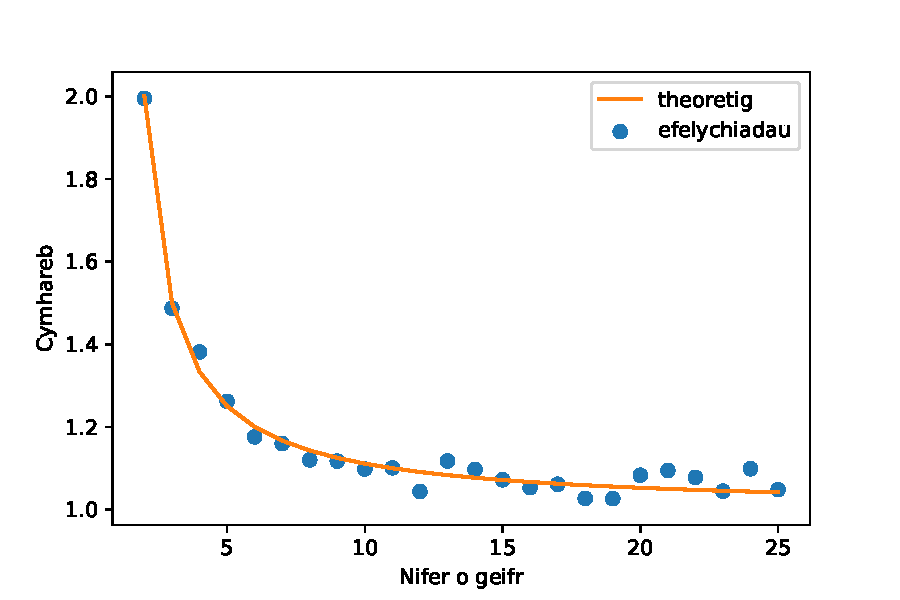
\includegraphics[width=.6\textwidth]{./simulated_v_expected_ratio_of_win_probability.pdf}
    \end{center}
    \caption{Yr effaith disgwyliedig ac o'r efelychiad o eifr ar y tebygolrwydd o ennill}
    \label{fig:simulated_v_expected_ratio_of_win_probability}
\end{figure}

Yn olaf gadewch i ni wirio wrth i nifer o eifr cynyddu mae'r effaith o newid yn
mynd yn llai ac yn llai:

\begin{multicols}{2}

    \begin{align}
        \lim_{n\to\infty}\alpha_n & = \lim_{n\to\infty}\frac{n}{n - 1}\\
        \lim_{n\to\infty}\alpha_n & = \lim_{n\to\infty}\frac{1}{1 - 1 / n}\\
        \lim_{n\to\infty}\alpha_n & = 1
    \end{align}

    \columnbreak

Yn defnyddio Python i wirio'r cyfrifiad:

    \begin{minted}{python}
    >>> import sympy as sym
    >>> alpha_n = p_n / (1 / (n + 1))
    >>> sym.limit(alpha_n, n, sym.oo)
    1
    \end{minted}

\end{multicols}

\section{Casgliad}

Mae'r adroddiad yma wedi defnyddio mathemateg a Python i uwcholeuo'r problem
Monty Hall. Mae fersiwn o'r g\^{e}m wedi addasu i ystyried r effaith o gael
unrhyw nifer o eifr yn y g\^{e}m.

Cawn fformiwla analytig ar gyfer y tebygolrwydd o ennill os yw'r cystadleuydd yn
newid.

Wrth i nifer y geifr cynyddu mae'r budd-effaith o newid yn lleihau: mae hwn yn
gwneud synnwyr oherwydd po fwyaf nifer y geifr, po leiaf yw effaith y cyflwynwr
yn dangos drws gyda gafr tu \^{o}l iddo.

Gall cyfeiriadau ymchwil eraill cynnwys edrych ar effaith ychwanegu mwy o geir,
a beth sy'n digwydd os yw'r cyflwynwr yn agor mwy o ddrysau gyda geifr tu \^{o}l
iddynt.


\bibliographystyle{plain}
\bibliography{bibliography.bib}

\end{document}
